% Appendix A

% \addcontentsline{toc}{section}{Appendix A}
\section{}
\label{app:appendix-a}


\newpage
\section{}
\label{app:appendix-b}

\begin{minted}[frame=single, framesep=2mm, baselinestretch=1.2, fontsize=\footnotesize, breaklines,linenos, numbersep=5pt]{text}
2023-12-27 23:22:26.546868:
(32, 64, 128, 128, 3, 3, 3, 3, 0.1, 0.0, 0.0, 512, 'adam', 32, 10) CHECKED
Best Score: 0.5725693106651306
Best Params: {'conv_1_filters': 32, 'conv_2_filters': 64, 'conv_3_filters': 128, 'conv_4_filters': 128, 'conv_1_kernel': 3, 'conv_2_kernel': 3, 'conv_3_kernel': 3, 'conv_4_kernel': 3, 'dropout_1': 0.1, 'dropout_2': 0.0, 'dropout_3': 0.0, 'dense_units': 512, 'optimizer': 'adam'}
(32, 64, 128, 128, 3, 3, 3, 3, 0.1, 0.0, 0.0, 768, 'adam', 32, 10) CHECKED
Best Score: 0.5725693106651306
Best Params: {'conv_1_filters': 32, 'conv_2_filters': 64, 'conv_3_filters': 128, 'conv_4_filters': 128, 'conv_1_kernel': 3, 'conv_2_kernel': 3, 'conv_3_kernel': 3, 'conv_4_kernel': 3, 'dropout_1': 0.1, 'dropout_2': 0.0, 'dropout_3': 0.0, 'dense_units': 512, 'optimizer': 'adam'}
2023-12-27 23:24:26.831029:
(32, 64, 128, 128, 3, 3, 3, 3, 0.1, 0.0, 0.0, 1024, 'adam', 32, 10) CHECKED
Best Score: 0.5765619874000549
Best Params: {'conv_1_filters': 32, 'conv_2_filters': 64, 'conv_3_filters': 128, 'conv_4_filters': 128, 'conv_1_kernel': 3, 'conv_2_kernel': 3, 'conv_3_kernel': 3, 'conv_4_kernel': 3, 'dropout_1': 0.1, 'dropout_2': 0.0, 'dropout_3': 0.0, 'dense_units': 1024, 'optimizer': 'adam'}
2023-12-27 23:25:37.281540:
(32, 64, 128, 128, 3, 3, 3, 3, 0.1, 0.0, 0.2, 512, 'adam', 32, 10) CHECKED
Best Score: 0.5906981825828552
Best Params: {'conv_1_filters': 32, 'conv_2_filters': 64, 'conv_3_filters': 128, 'conv_4_filters': 128, 'conv_1_kernel': 3, 'conv_2_kernel': 3, 'conv_3_kernel': 3, 'conv_4_kernel': 3, 'dropout_1': 0.1, 'dropout_2': 0.0, 'dropout_3': 0.2, 'dense_units': 512, 'optimizer': 'adam'}
2023-12-27 23:26:47.249360: 
(32, 64, 128, 128, 3, 3, 3, 3, 0.1, 0.0, 0.2, 768, 'adam', 32, 10) CHECKED
Best Score: 0.5906981825828552
Best Params: {'conv_1_filters': 32, 'conv_2_filters': 64, 'conv_3_filters': 128, 'conv_4_filters': 128, 'conv_1_kernel': 3, 'conv_2_kernel': 3, 'conv_3_kernel': 3, 'conv_4_kernel': 3, 'dropout_1': 0.1, 'dropout_2': 0.0, 'dropout_3': 0.2, 'dense_units': 512, 'optimizer': 'adam'}
2023-12-27 23:27:57.635618: 
(32, 64, 128, 128, 3, 3, 3, 3, 0.1, 0.0, 0.2, 1024, 'adam', 32, 10) CHECKED
Best Score: 0.5906981825828552
Best Params: {'conv_1_filters': 32, 'conv_2_filters': 64, 'conv_3_filters': 128, 'conv_4_filters': 128, 'conv_1_kernel': 3, 'conv_2_kernel': 3, 'conv_3_kernel': 3, 'conv_4_kernel': 3, 'dropout_1': 0.1, 'dropout_2': 0.0, 'dropout_3': 0.2, 'dense_units': 512, 'optimizer': 'adam'}
2023-12-27 23:29:09.047680:
(32, 64, 128, 128, 3, 3, 3, 3, 0.1, 0.0, 0.3, 512, 'adam', 32, 10) CHECKED
Best Score: 0.5906981825828552
Best Params: {'conv_1_filters': 32, 'conv_2_filters': 64, 'conv_3_filters': 128, 'conv_4_filters': 128, 'conv_1_kernel': 3, 'conv_2_kernel': 3, 'conv_3_kernel': 3, 'conv_4_kernel': 3, 'dropout_1': 0.1, 'dropout_2': 0.0, 'dropout_3': 0.2, 'dense_units': 512, 'optimizer': 'adam'}
2023-12-27 23:30:18.471026:
(32, 64, 128, 128, 3, 3, 3, 3, 0.1, 0.0, 0.3, 768, 'adam', 32, 10) CHECKED
Best Score: 0.5906981825828552
Best Params: {'conv_1_filters': 32, 'conv_2_filters': 64, 'conv_3_filters': 128, 'conv_4_filters': 128, 'conv_1_kernel': 3, 'conv_2_kernel': 3, 'conv_3_kernel': 3, 'conv_4_kernel': 3, 'dropout_1': 0.1, 'dropout_2': 0.0, 'dropout_3': 0.2, 'dense_units': 512, 'optimizer': 'adam'}
\end{minted}

\newpage

\section{}
\label{app:appendix-c}
\begin{figure}[h!]
    \centering
    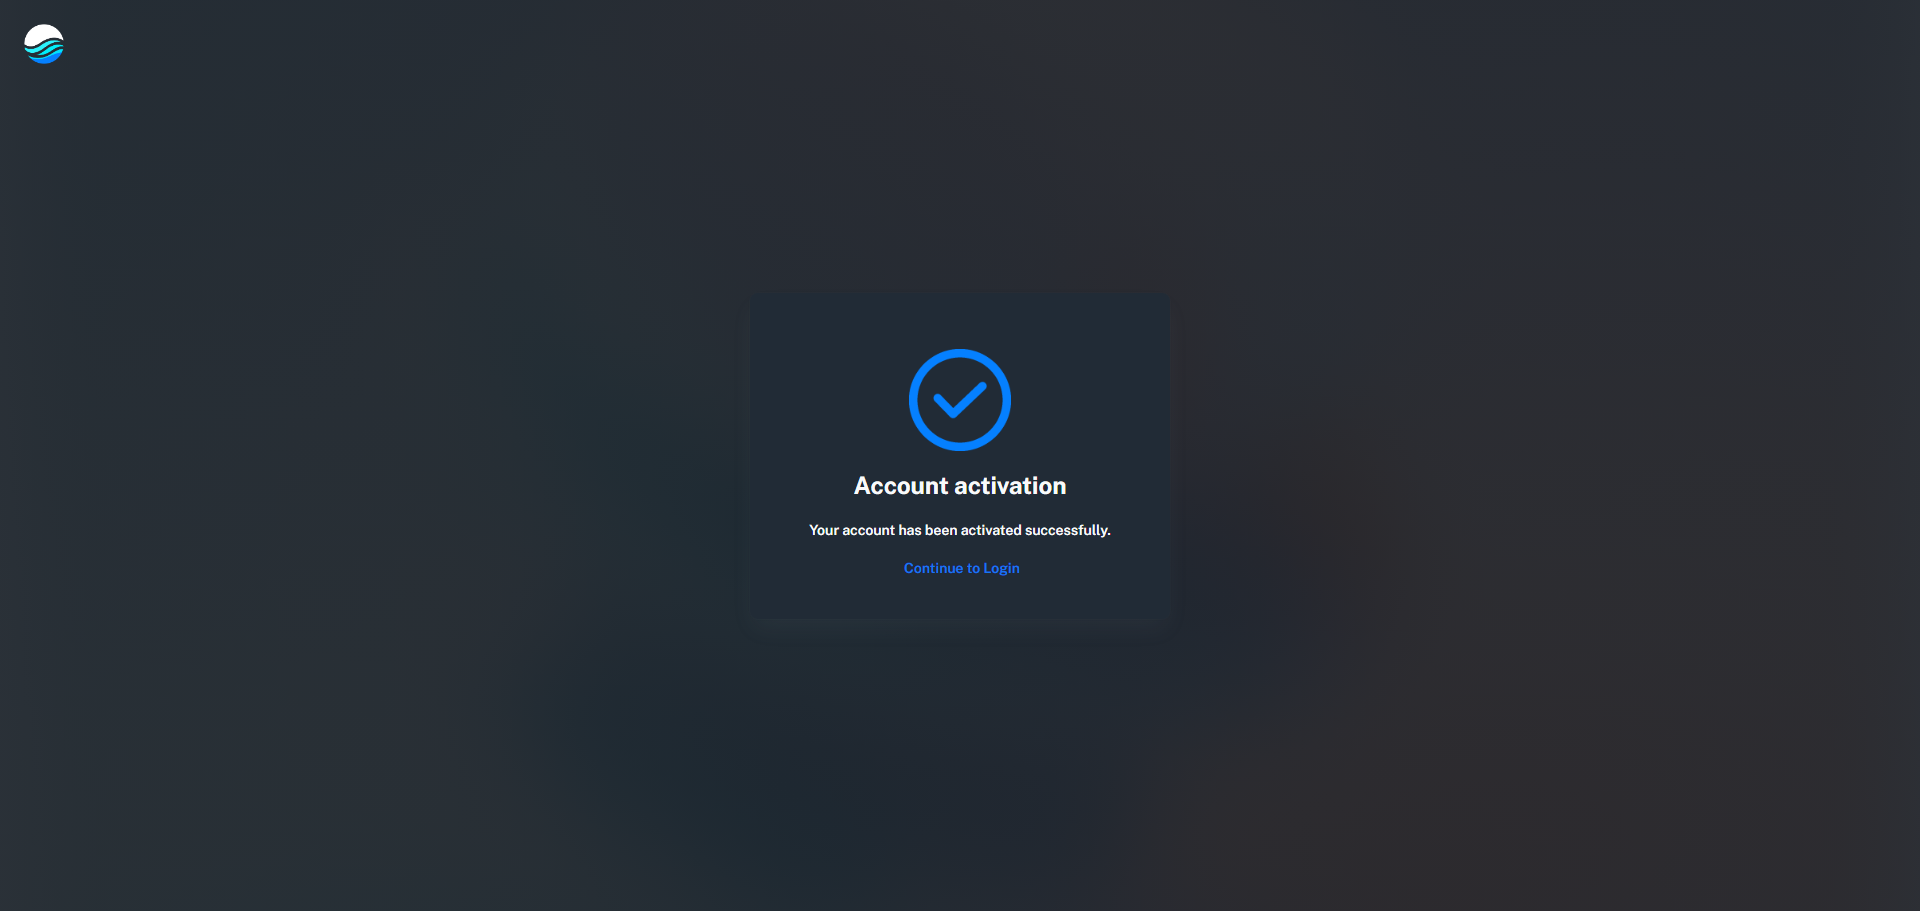
\includegraphics[width=14cm]{Images/acc-activated.png}
    \caption{Account Activated - UI}
    \label{fig:acc-activated}
\end{figure}
\begin{figure}[h!]
    \centering
    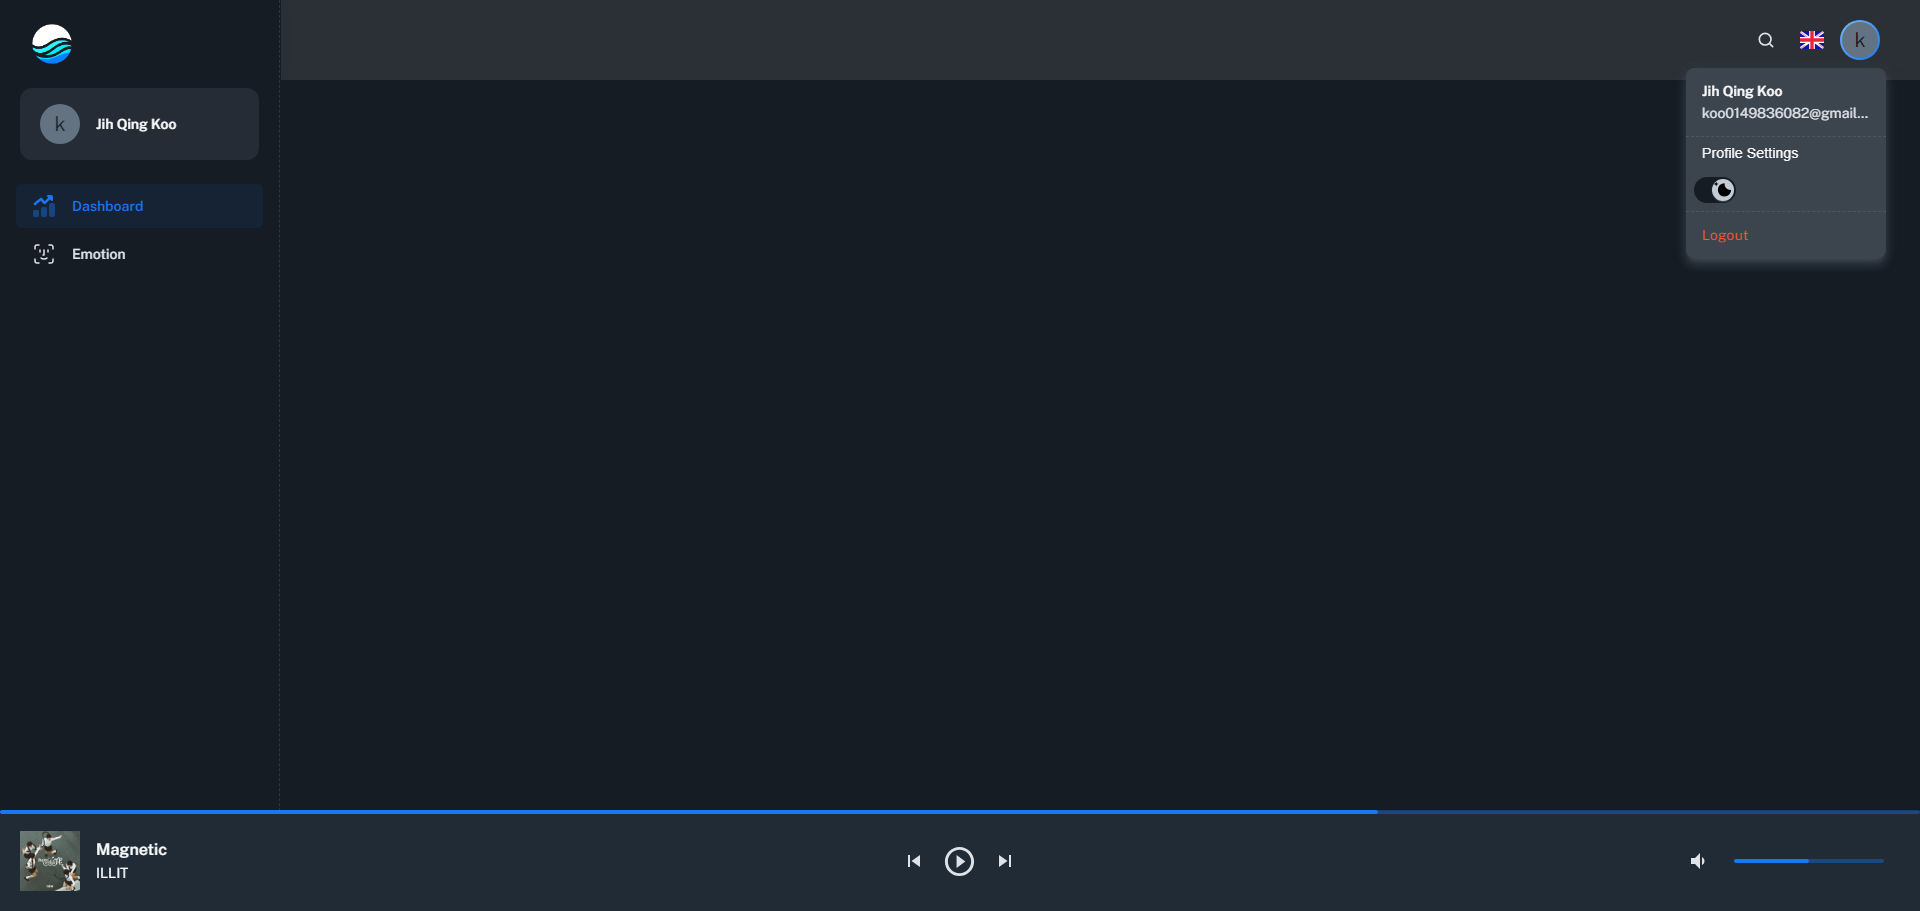
\includegraphics[width=14cm]{Images/dashboard.png}
    \caption{Dashboard - UI}
    \label{fig:dashboard-ui}
\end{figure}
\begin{figure}[h!]
    \centering
    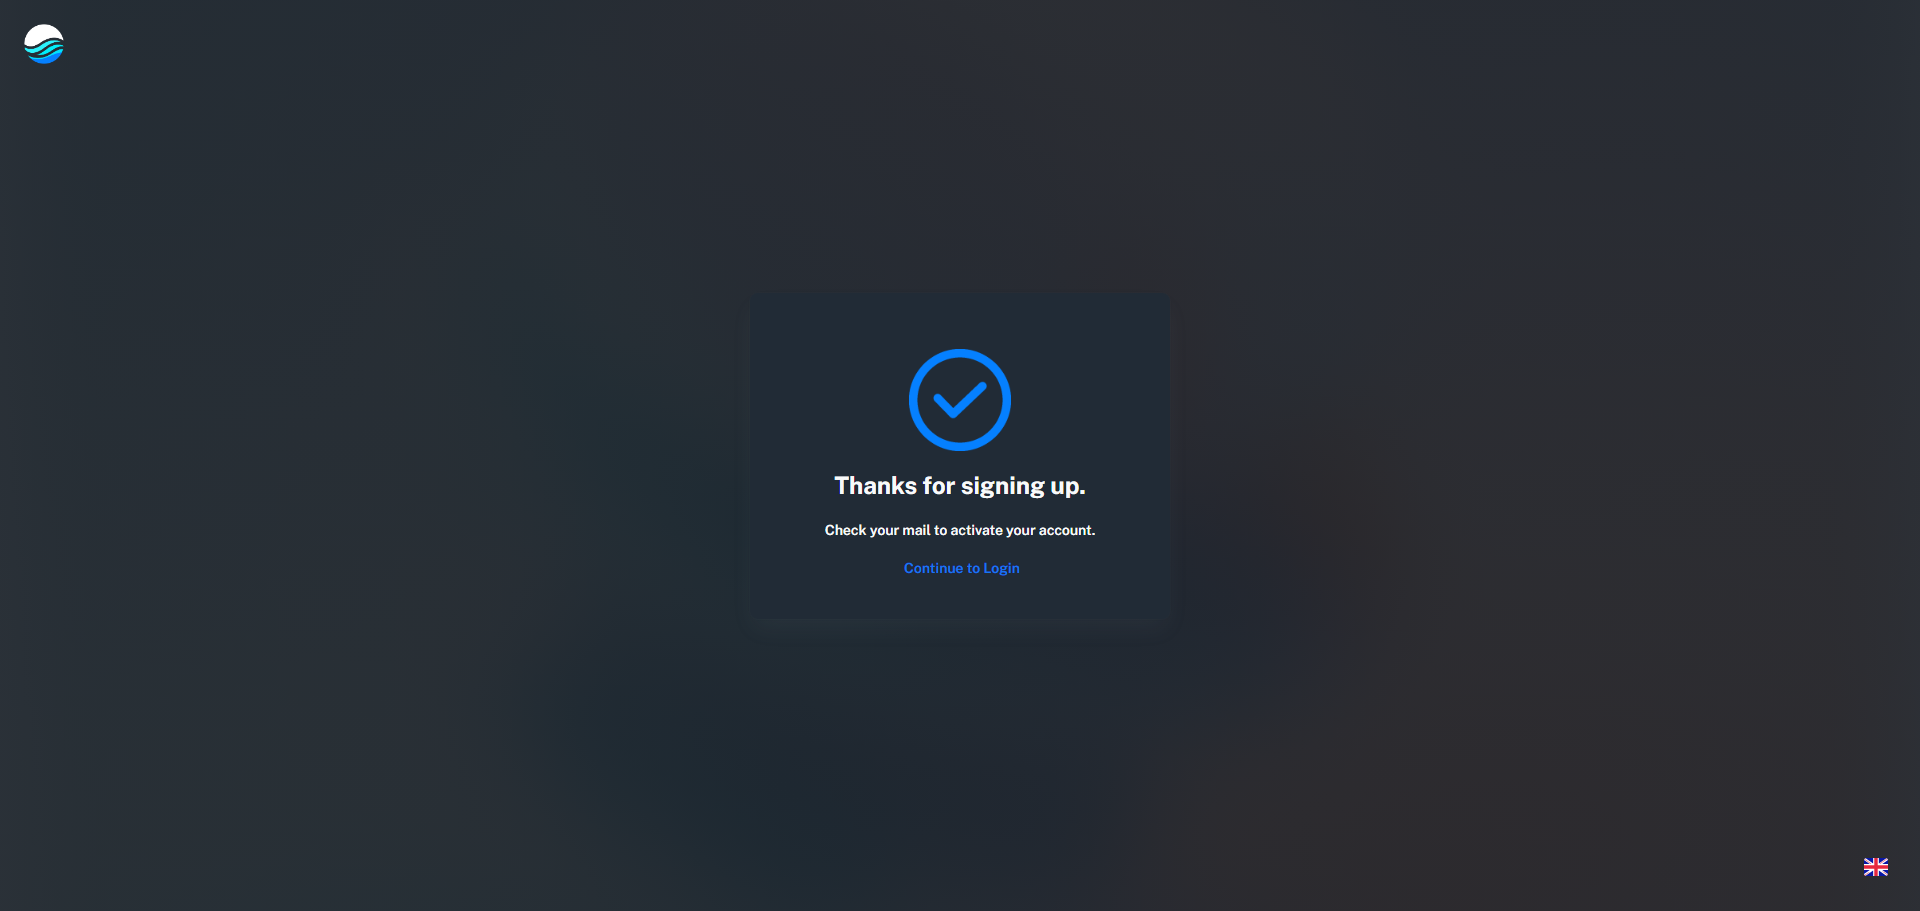
\includegraphics[width=14cm]{Images/register-successfull-ui.png}
    \caption{Register Successful - UI}
    \label{fig:register-succesfull}
\end{figure}
\begin{figure}[h!]
    \centering
    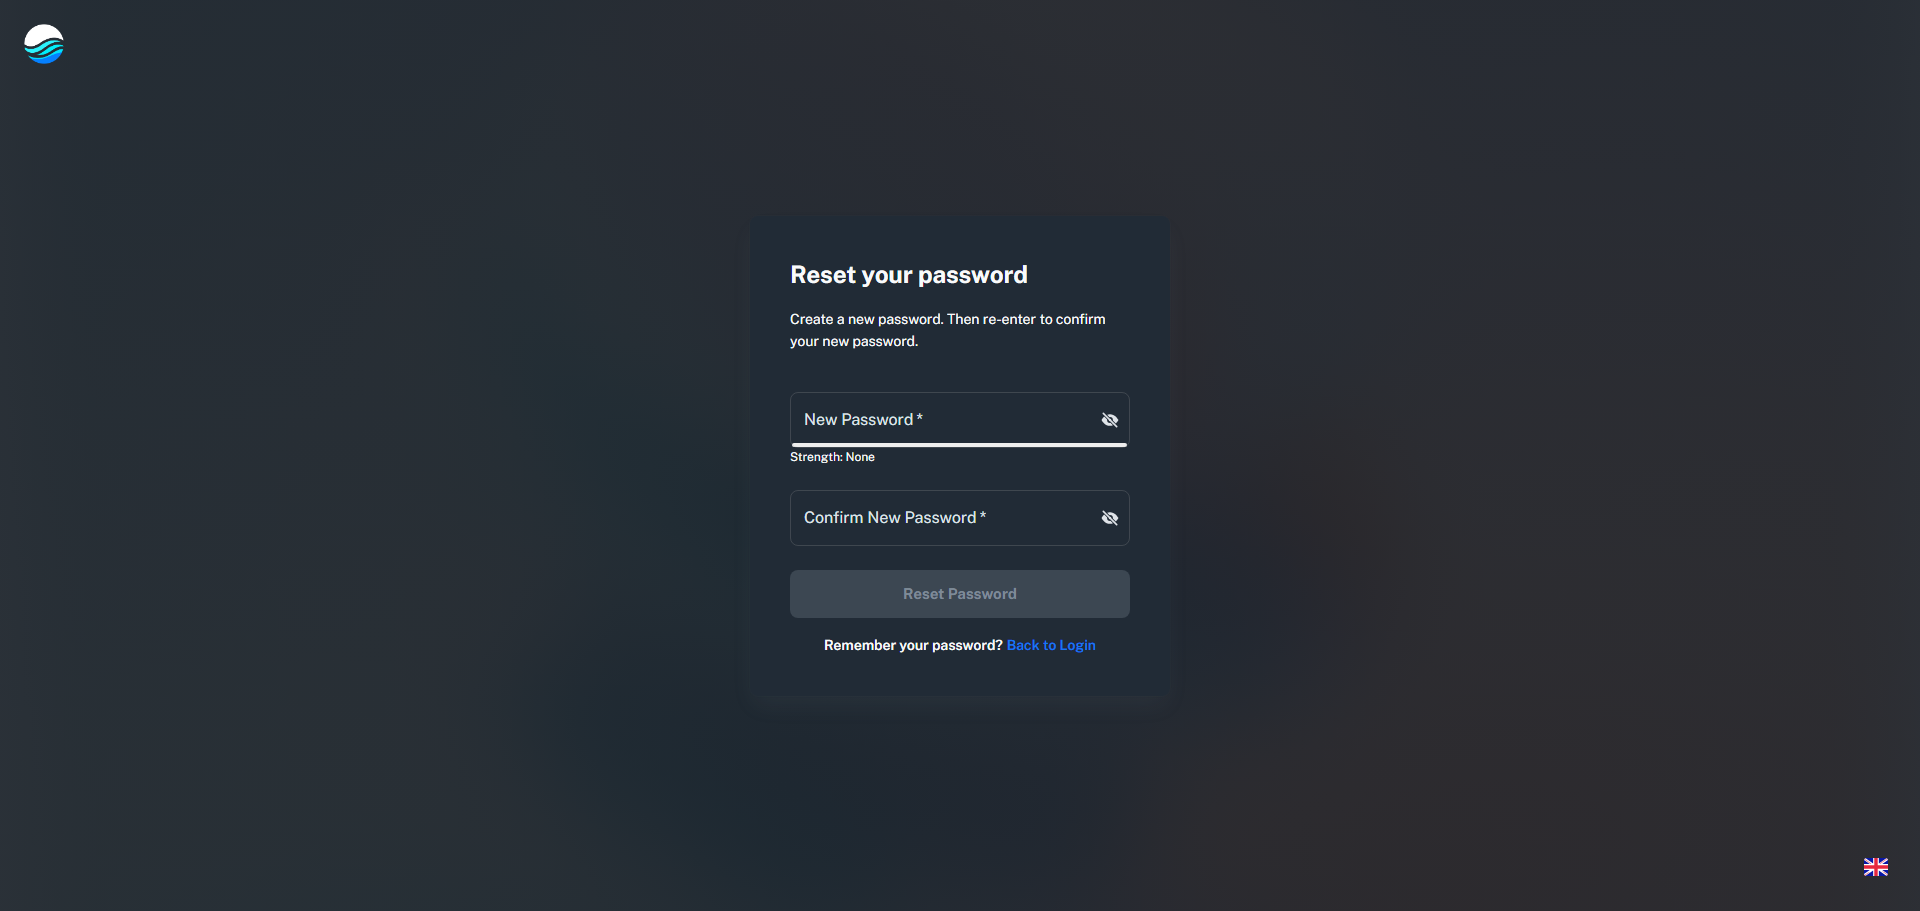
\includegraphics[width=14cm]{Images/reset-password-ui.png}
    \caption{Reset Password - UI}
    \label{fig:reset-password-ui}
\end{figure}
\begin{figure}[htbp]
    \centering
    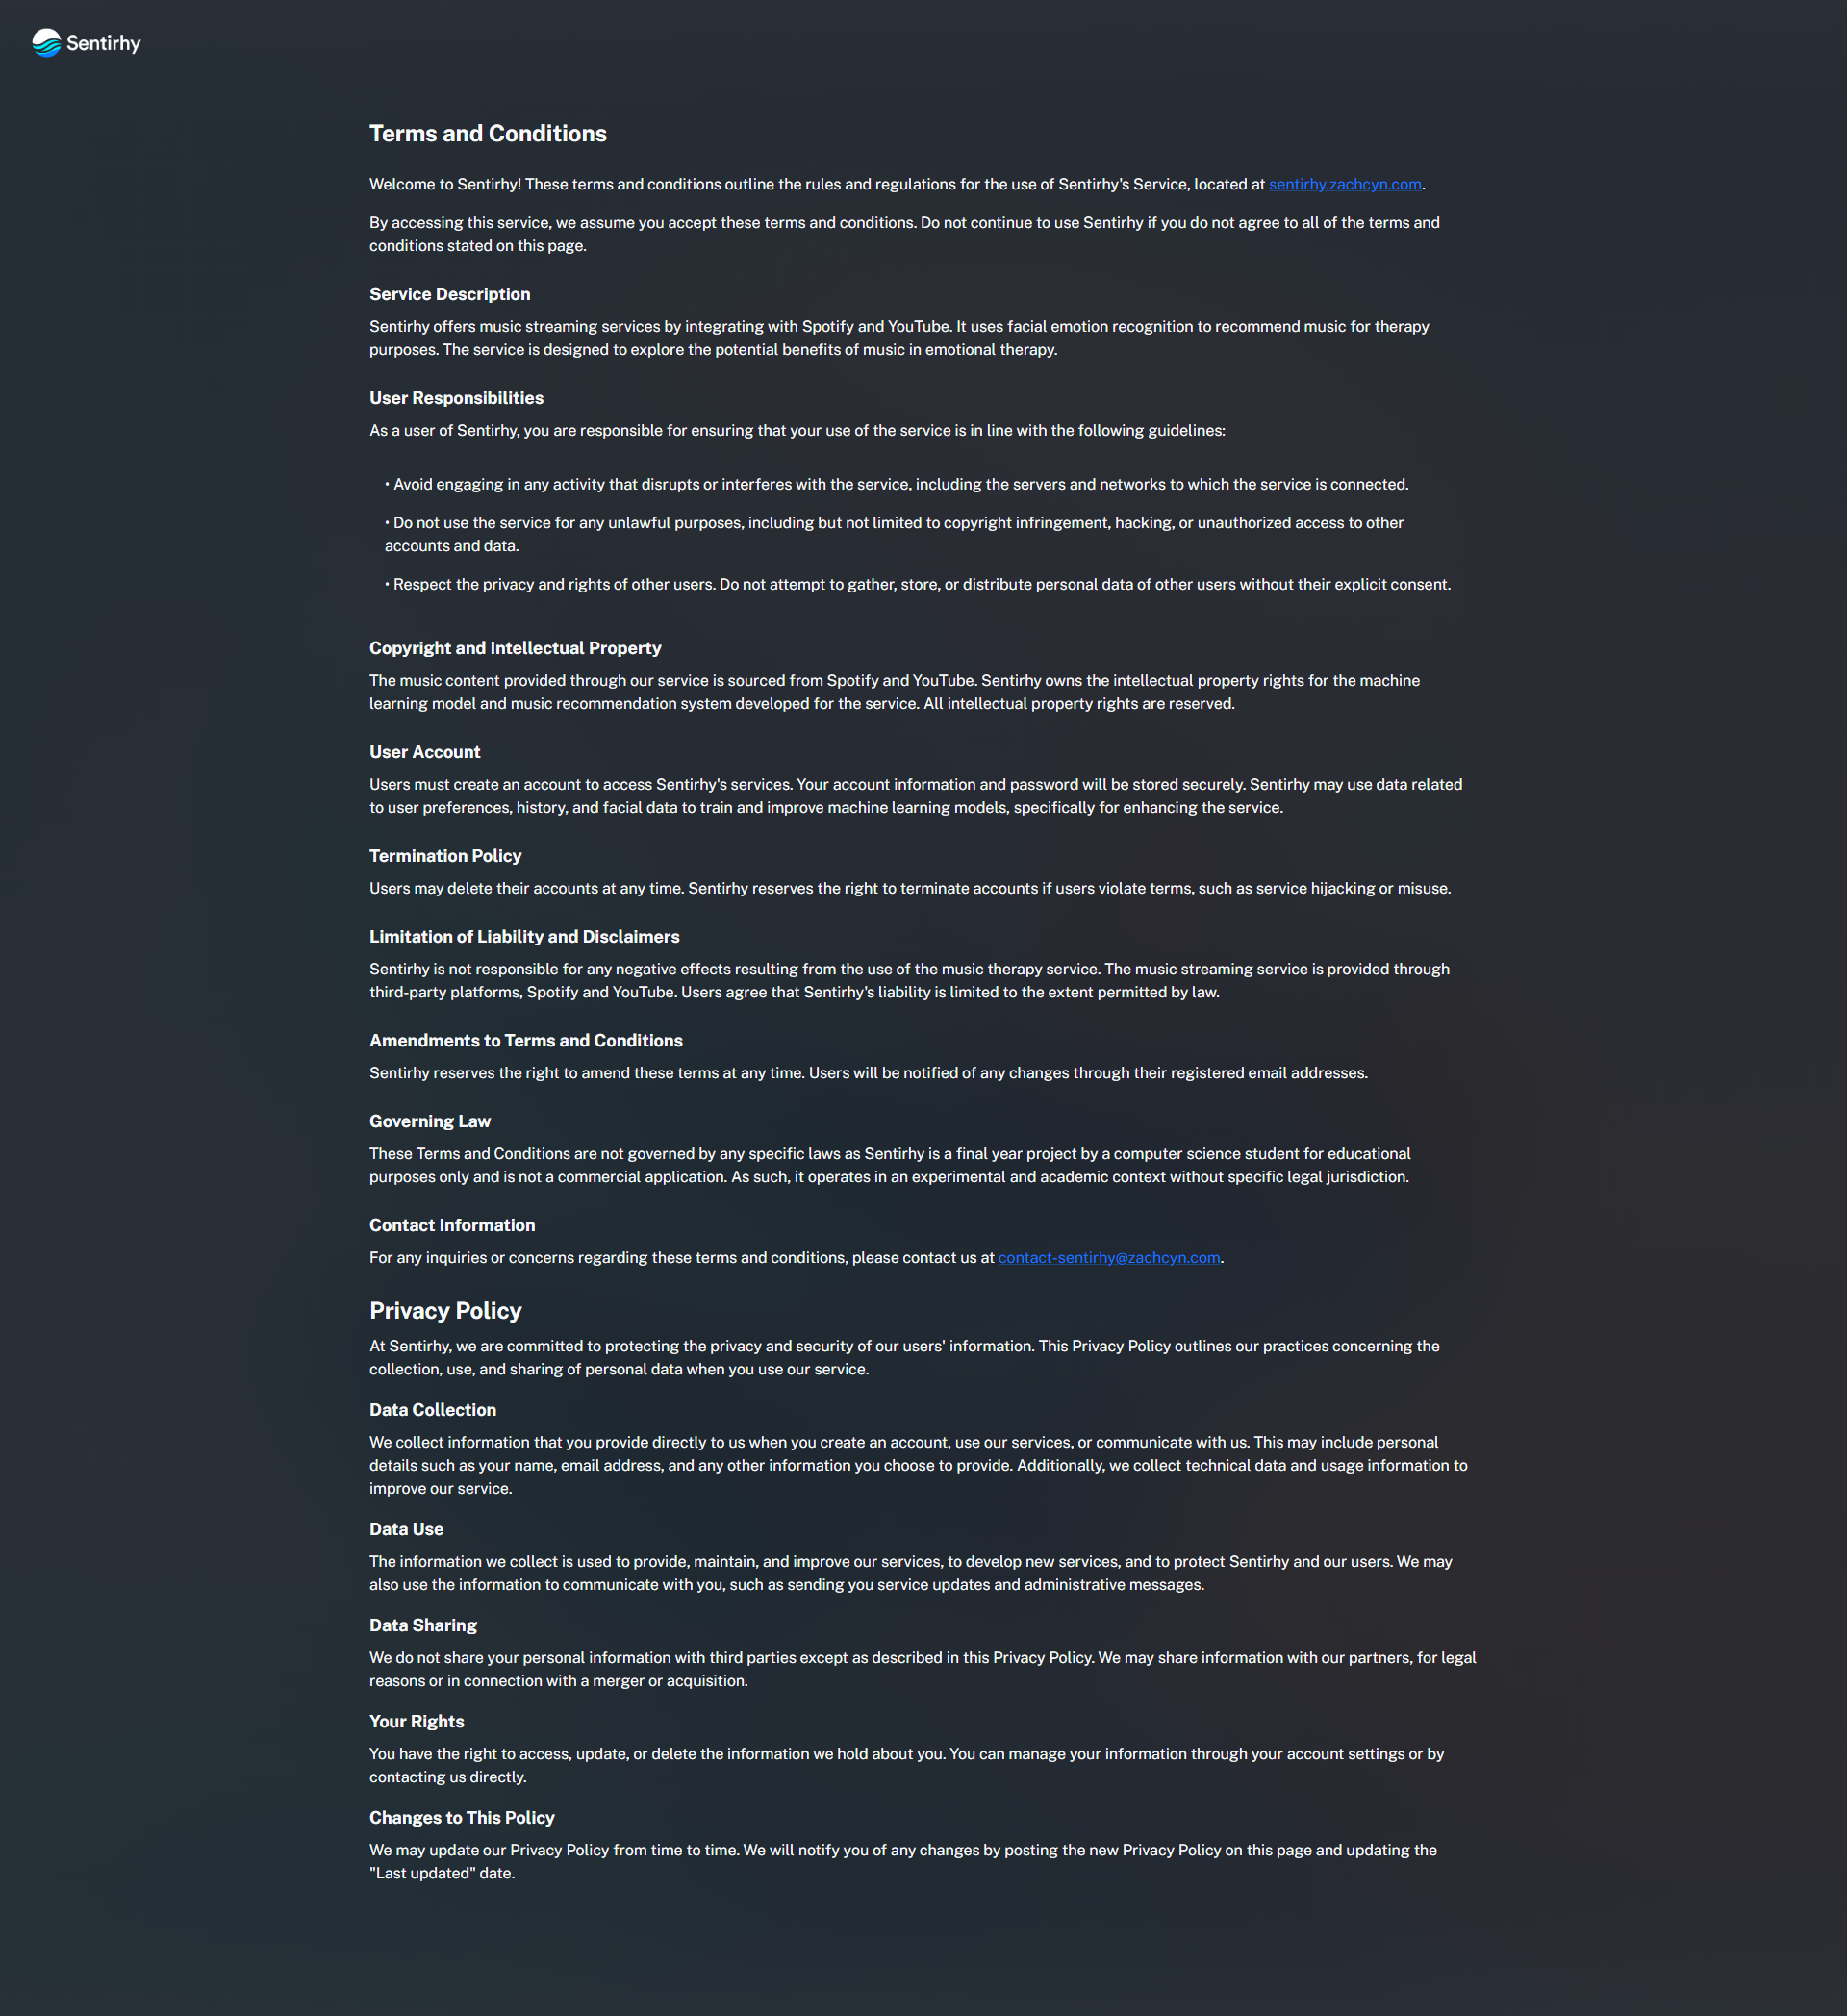
\includegraphics[width=0.75\textwidth]{Images/t_and_c-ui.png}
    \caption{Terms and Conditions - UI}
    \label{fig:terms}
  \end{figure}
\begin{figure}[h!]
    \centering
    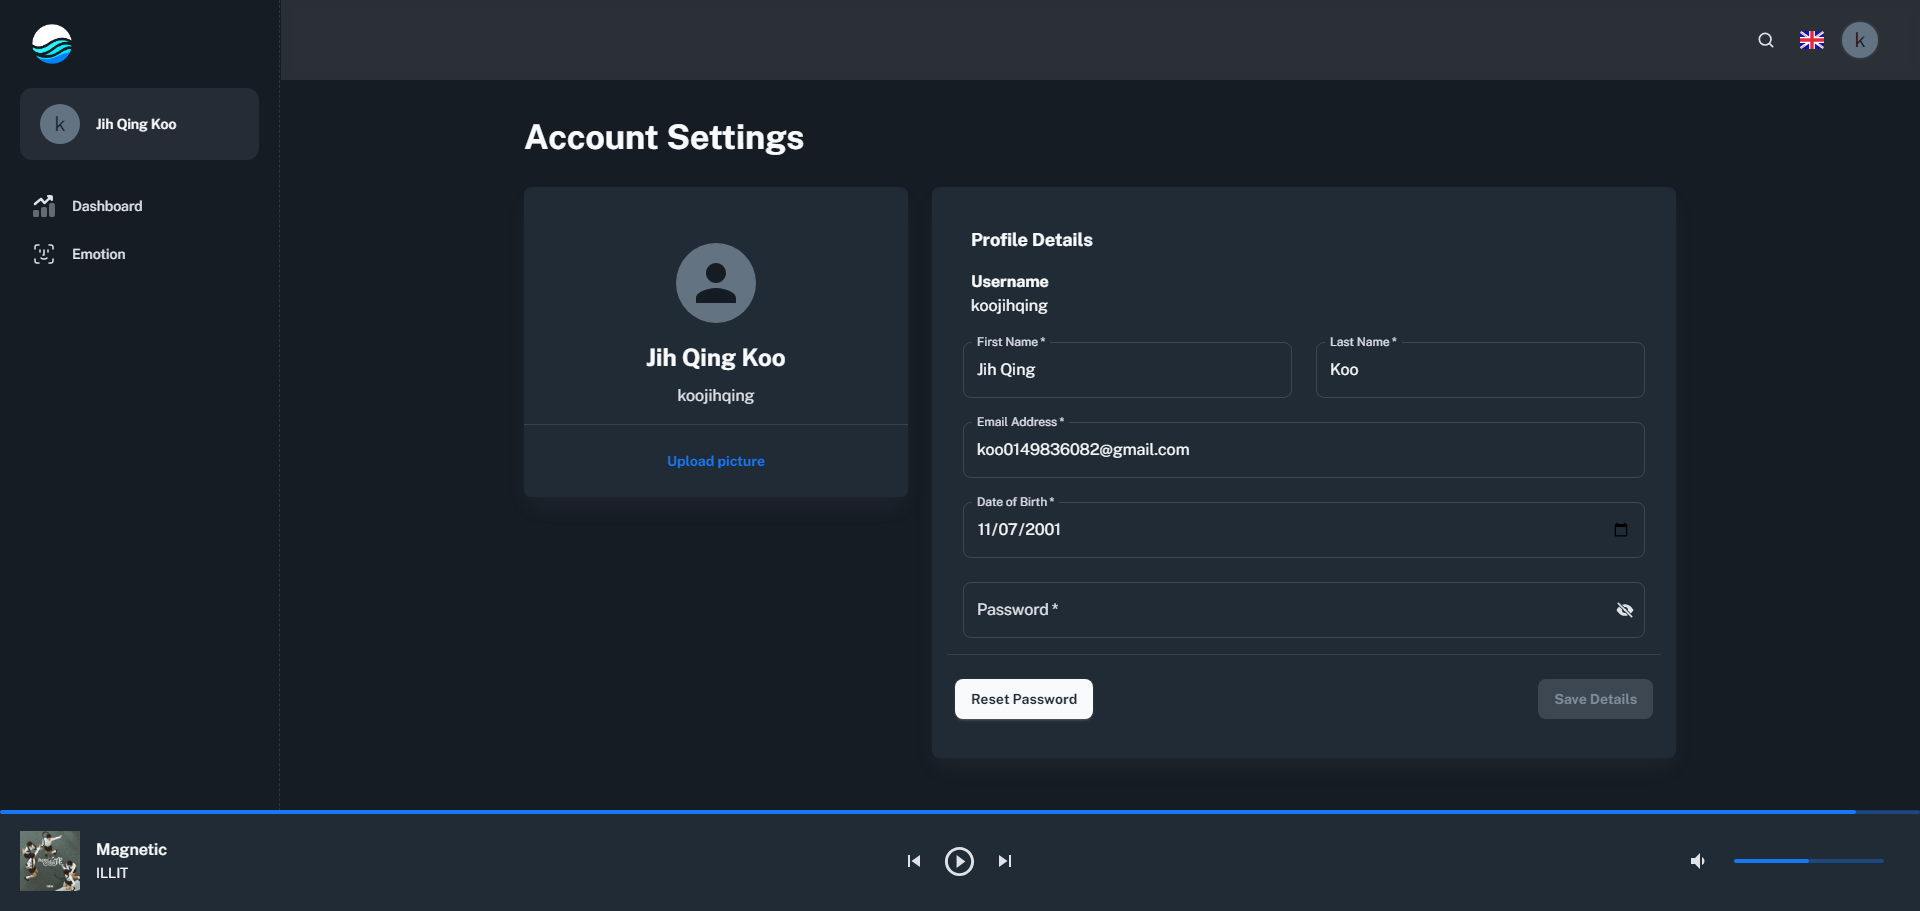
\includegraphics[width=14cm]{Images/user-settings-ui.png}
    \caption{User Settings - UI}
    \label{fig:user-settings-ui}
\end{figure}

\newpage
\begin{landscape}
\section{}
\label{app:appendix-d}
\begin{longtable}{ |m{1cm}|m{1.5cm}|m{5cm}|m{6cm}|m{6cm}|m{2cm}| }
    \hline
    \rowcolor{lightgray}
    \textbf{Test No.} & \textbf{Cats.} & \textbf{Intention} & \textbf{Expected Result} & \textbf{Actual Result} & \textbf{Pass/Fail} \\
    \hline
    \endfirsthead

    \hline
    \rowcolor{lightgray}
    \textbf{Test No.} & \textbf{Cats.} & \textbf{Intention} & \textbf{Expected Result} & \textbf{Actual Result} & \textbf{Pass/Fail} \\
    \hline
    \endhead
    1 & \gls{ui} & Registration & User registered & User registered and information added to database & Pass \\
    \hline
    2 & \gls{ui} & Login & User logged in & User logged in successfully & Pass \\
    \hline
    3 & \gls{ui} & Incorrect credentials upon login & User login failed and error message display & Error message displayed and user unable to login & Pass \\
    \hline
    4 & \gls{ui} & Account Activation & User received email and activate account from link & User activate account successfully from link & Pass \\
    \hline
    5 & \gls{ui} & Reset Password without Authentication & Reset link sent to user, and password reset successfully & Link sent, password reset successfully & Pass \\
    \hline
    6 & \gls{ui} & Connect Spotify API & Redirect user to Spotify Authentication Page, and redirect back to `Dashboard' & Granted permission from Spotify and brought user back to `Dashboard' & Pass \\
    \hline
    7 & \gls{ui} & Connect Youtube API & Redirect user to Youtube Authentication Page, and redirect back to `Dashboard' & Youtube API connection not implemented & Fail \\
    \hline
    8 & \gls{ui} & Play Music & Music play through Web Playback & Music played & Pass \\
    \hline
    9 & \gls{ui} & Skip Music & Skip music through Web Playback & Music skipped & Pass \\
    \hline
    10 & \gls{ui} & Previous Music & Play previous music through Web Playback &  Previous Music played & Pass \\
    \hline
    11 & \gls{ui} & Adjust Volume & Volume higher or lower & Volume does adjusted through the slider & Pass \\
    \hline
    12 & \gls{ui} & Mute & Mute Web Playback & Music does muted & Pass \\
    \hline
    13 & \gls{ui} & Toggle light/dark theme & Theme switched when user pressed the button & Theme switched & Pass \\
    \hline
    14 & \gls{ui} & Detect user's system theme & Theme detected and switched to user's system theme & Theme switched accordingly & Pass \\
    \hline
    15 & \gls{ui} & Switch language & Web application language switched to user's preferred language & Language switched & Pass\\
    \hline
    16 & \gls{ui} & Change personal details in Settings & Update entered details to database & User's information is updated & Pass\\
    \hline
    17 & \gls{ui} & Change profile picture in Settings & Saved image to server and update the file path to database & Image saved and database updated & Pass\\
    \hline
    18 & \gls{ui} & Reset Password in Settings & Update new password to database & New password saved in database with encrypted & Pass \\
    \hline
    19 & \gls{ui} & Capture user's frame when face detected & Frame captured & Frame Captured with face showed clearly & Pass \\
    \hline
    20 & \gls{ml} & Emotion Detection & Emotion detected on the captured frame & Emotion detected & Pass \\
    \hline
    21 & \gls{ui} & Display recognized emotion on \gls{ui} & Detected emotion is showed on user's screen & Detected emotion showing on user's screen & Pass \\
    \hline
    22 & Server & Generate playlist & Generate playlist based on user's current emotion & Playlist generated based on user's current emotion & Pass \\
    \hline
    23 & \gls{ui} & Logout & User logged out, authentication token removed & Token removed and user logged out & Pass \\
    \hline
    \caption{Test Table}
\end{longtable}
\end{landscape}

\newpage
\begin{landscape}
\section{}
\label{app:appendix-e}
\begin{longtable}{ |m{2.5cm}|m{2.5cm}|m{2cm}|m{6.5cm}|m{8cm}| }
    \hline
    \rowcolor{lightgray}
    \textbf{Date} & \textbf{Time} & \textbf{Location} & \textbf{Title} & \textbf{Attendees} \\
    \hline
    \endfirsthead

    \hline
    \rowcolor{lightgray}
    \textbf{Date} & \textbf{Time} & \textbf{Location} & \textbf{Title} & \textbf{Attendees} \\
    \hline
    \endhead
    16-10-2023 & 1505-1700 & X Block & Project Idea and Aim Discussion & Yie Nian Chu, Ali Suhail, Martin Serpell \\
    \hline
    17-10-2023 & 1500-1515 & 2Q17 & Project Idea and Aim Discussion & Yie Nian Chu, Craig Duffy \\
    \hline
    23-10-2023 & 1505-1605 & X Block & Project Idea and Aim Disucssion & Yie Nian Chu, Ali Suhail, Martin Serpell \\
    \hline
    25-10-2023 & 1400-1430 & Microsoft Teams & Final Decision on Project Idea & Yie Nian Chu, Craig Duffy \\
    \hline
    30-10-2023 & 1505-1520 & X Block & Project Discussion & Yie Nian Chu, Ali Suhail, Martin Serpell \\
    \hline
    22-11-2023 & 1000-1030 & Microsoft Teams & Progress Follow Up (Lit. Review) & Yie Nian Chu, Craig Duffy \\
    \hline
    06-12-2023 & 1000-1020 & Microsoft Teams & Progress Follow Up (Lit. Review) & Yie Nian Chu, Craig Duffy \\
    \hline
    12-12-2023 & 1330-1400 & 2Q17 & Development Discussion & Yie Nian Chu, Craig Duffy \\
    \hline
    16-01-2024 & 1500-1530 & Microsoft Teams & Project Poster Discussion & Yie Nian Chu, Joseph Cauvy-Foster, Craig Duffy \\
    \hline
    06-02-2024 & 1600-1630 & 2Q17 & Progress Follow Up (Dev) & Yie Nian Chu, Craig Duffy \\
    \hline
    05-03-2024 & 1200-1215 & 2Q17 & Progress Follow Up (Dev) & Yie Nian Chu, Craig Duffy \\
    \hline
    \caption{Meeting Log}
\end{longtable}
\end{landscape}